% Requires graphicx; Tables 1--3 additionally require booktabs.
% Copy the generated figures/ directory alongside the manuscript .tex file.
\begin{figure*}[t]
  \centering
  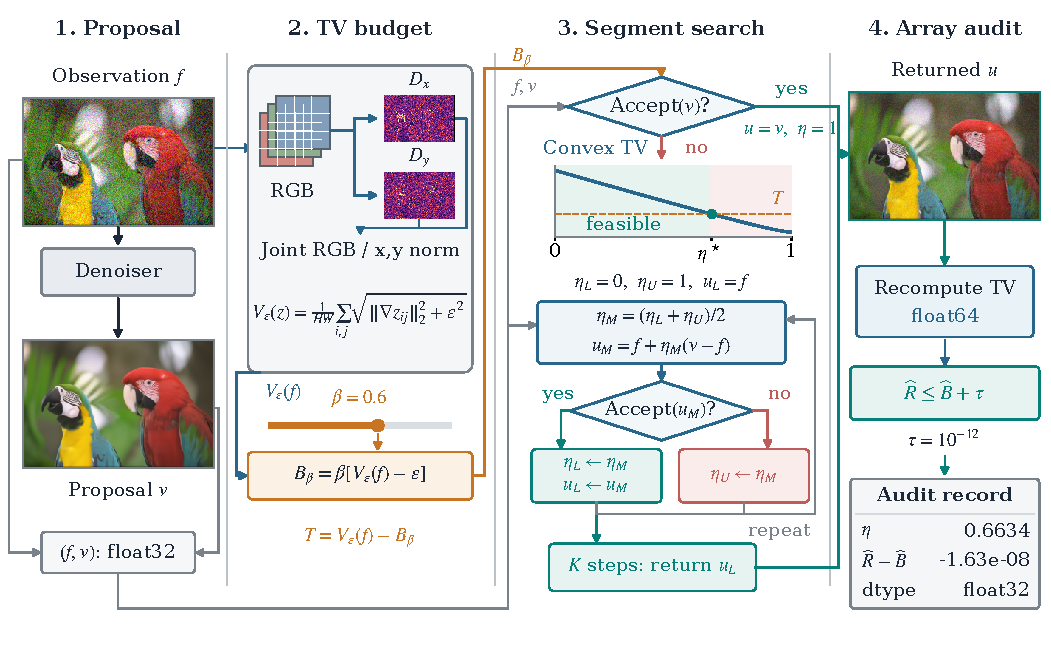
\includegraphics[width=\textwidth]{figures/ICASSP_Overview_Technical.pdf}
  \caption{Overview of the TV-budget controller.}
  \label{fig:overview}
\end{figure*}

\begin{figure}[t]
  \centering
  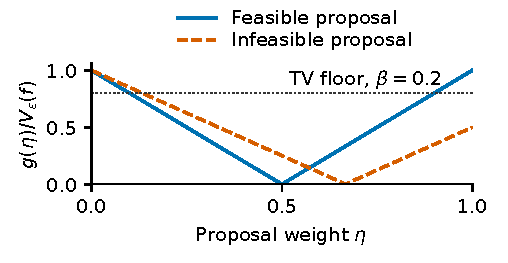
\includegraphics[width=\columnwidth]{figures/geometry.pdf}
  \caption{Nonmonotone segment TV for $f=(0.1,0.9)$ repeated in RGB.
  Proposal $(0.9,0.1)$ has a feasible endpoint but an infeasible middle;
  $(0.7,0.3)$ has a feasible prefix supporting bisection.}
  \label{fig:geometry}
\end{figure}

\begin{figure}[t]
  \centering
  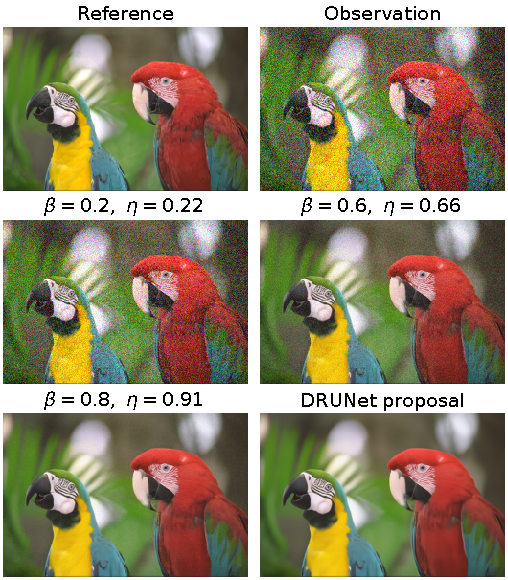
\includegraphics[width=\columnwidth]{figures/visual_single_column.pdf}
  \caption{Budget-controlled outputs for Kodak kodim23 at $\sigma=25/255$,
  using the same observation and DRUNet proposal. Full resized images use
  identical display scaling.}
  \label{fig:visual}
\end{figure}

\begin{figure}[t]
  \centering
  \begin{minipage}[t]{0.49\columnwidth}
    \centering
    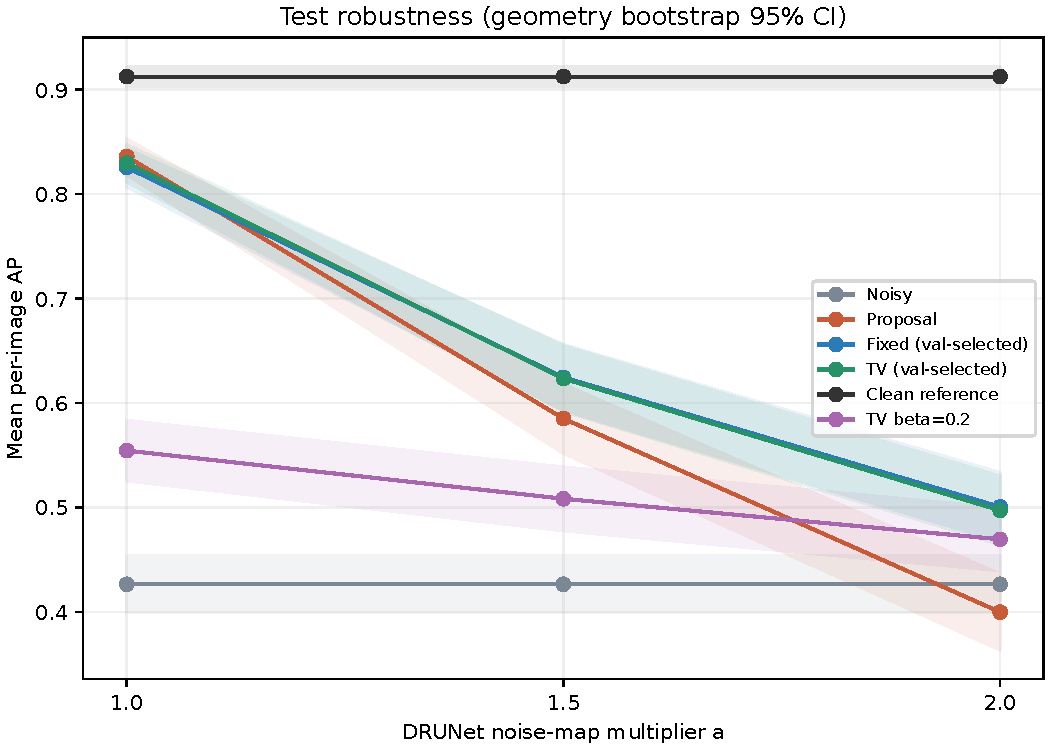
\includegraphics[width=\linewidth]{figures/test_robustness.pdf}
    \par\small (a) Denoising mismatch.
  \end{minipage}\hfill
  \begin{minipage}[t]{0.49\columnwidth}
    \centering
    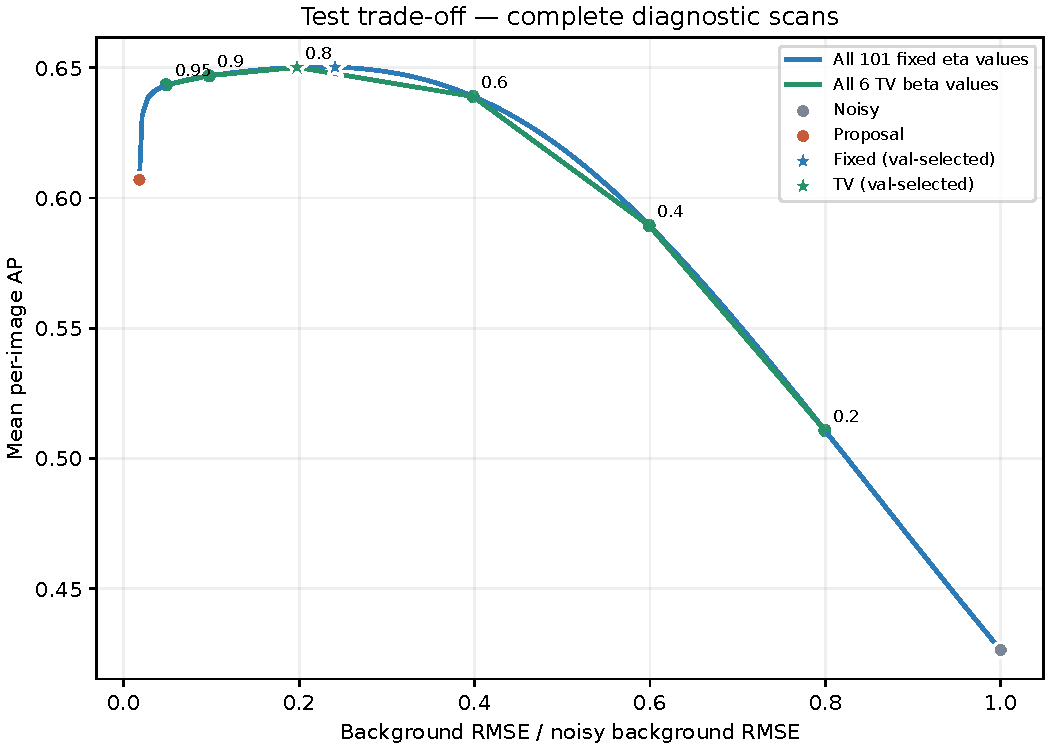
\includegraphics[width=\linewidth]{figures/test_tradeoff.pdf}
    \par\small (b) Detection--noise trade-off.
  \end{minipage}
  \caption{Weak-structure detection on 100 held-out test geometries.
  (a) Mean AP versus noise-map multiplier $a$; shading indicates
  geometry-bootstrap 95\% CIs. (b) Complete fixed-blend and TV-budget scans,
  averaged over noise levels, repeats, and mismatch conditions. Stars mark
  validation-selected shared operating points; $\beta=0.2$ is also labeled.}
  \label{fig:weak_structure}
\end{figure}

\begin{figure}[t]
  \centering
  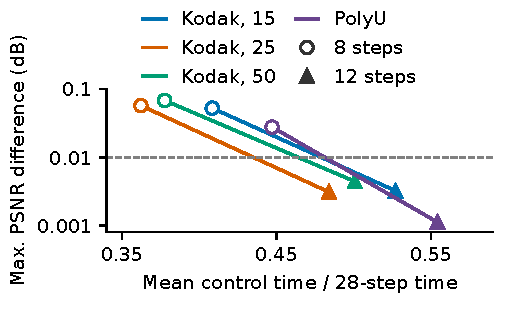
\includegraphics[width=\columnwidth]{figures/precision.pdf}
  \caption{Precision--cost trade-off relative to 28-step bisection across
  four budgets. Time is the ratio of mean condition-median times; quality
  is the maximum per-image absolute PSNR difference across the same
  conditions. Kodak labels denote $255\sigma$.}
  \label{fig:precision}
\end{figure}
